%!TEX root =  main.tex
\section{Background}
\label{sec:background}

\dynastar builds on state machine replication and scalable state machine replication.
In this section, we recall these techniques and the dynamic partitioning scheme proposed by Long et al.~\cite{hoang2016}.

\subsection{State Machine Replication}
\label{sec:smr}

State machine replication is a fundamental approach to implementing fault-tolerant services by replicating servers, and coordinating the execution of client commands at server replicas~\cite{Lam78,Sch90}. 
SMR ensures linearizability~\cite{Attiya04} by coordinating the execution of commands in the different replicas: 
Every replica has a full copy of the objects that compose the service state $\vvm = \{o_1, ..., o_m\}$ and executes commands submitted by the clients in the same order. 
A command is a program consisting of a sequence of operations, which can be of three types: $read(v)$, $write(v, val)$, or a deterministic computation.

By starting in the same initial state and executing the same sequence of deterministic commands, servers make the same state changes and produce the same reply for each command. To guarantee that servers deliver the same sequence of commands, SMR can be implemented with atomic broadcast: commands are atomically broadcast to all servers, and all correct servers deliver and execute the same sequence of commands \cite{BJ87b,DSU04}.

Despite its simple execution model, classical SMR does not scale: adding resources (e.g., replicas) will not translate into sustainable improvements in throughput. 
%This happens for two reasons. 
%First, the underlying communication protocol needed to ensure ordered message delivery may itself not scale (i.e., a communication bottleneck). 
%Second, every command must be executed sequentially by each replica (i.e., an execution bottleneck).
%
Several approaches have been proposed to address SMR's scalability limitations. 
In the following, we review Scalable State Machine Replication (\ssmr), an approach that partitions the service's state and replicates each partition (e.g., \cite{Glendenning:2011kj,Marandi:2011dj,hoang2016}).


\subsection{S-SMR with static partitioning}
\label{sec:ssmr}

%
%To cope with communication overhead, some proposals have suggested to spread the load of ordering commands among multiple processes (e.g., \cite{Moraru:2013gw,Mencius,Marandi:2012hb}), as opposed to dedicating a single process to determine the order of commands (e.g., \cite{Lamport:1998ea}).%\fxnote[draft]{remove inapplicable reference}
%
%Two directions of research have been suggested to overcome execution bottlenecks. One approach (scaling up) is to take advantage of multiple cores to execute commands concurrently without sacrificing consistency \cite{Kapritsos:2012um,Marandi:2014bj,Kotla:2004ep,Guo:2014jp}.
%% Remove candidate: END
%Another approach (scaling out) is to partition the service's state and replicate each partition (e.g., \cite{Glendenning:2011kj,Marandi:2011dj}). 
%In the next few sections, we review Scalable State Machine Replication (\ssmr) and its dynamic-partitioning variant \dssmr, both proposals related to scaling out the state.
%
In S-SMR~\cite{bezerra2014ssmr}, the service state \vvt\ is composed of $k$ partitions, $\ppm_1, ..., \ppm_k$, where each partition $\ppm_i$ is statically assigned to server group $\ssm_i$. 
For brevity, we say that server $s$ belongs to $\ppm_i$ meaning that $s \in \ssm_i$, and say ``multicast to $\ppm_i$" meaning ``multicast to server group $\ssm_i$".
S-SMR relies on an \emph{oracle}, which tells which partitions are accessed by each command.
%\footnote{The oracle returns a set with the partitions accessed by the command, but this set does not need to be minimal; it may contain all partitions in the worst case, when the partitions accessed by the command cannot be determined before the command is executed.}

To execute a command, a client multicasts the command to the appropriate partitions, as determined by the oracle.
Commands that access a single partition are executed as in classical SMR: replicas of the concerned partition agree on the execution order and each replica executes the command independently.
In the case of a multi-partition command, replicas of the involved partitions deliver the command and then may need to exchange state, since some partitions may not have all the values read in the command.
This mechanism allows commands to execute seamlessly despite the partitioned state.

%\begin{algorithm}[t!]
\small

\begin{distribalgo}[1]

\vspace{1mm}

\INDENT{\emph{Initialization:}}
    \STATE $\forall C \in $ \kk $ : rcvd\_signals(C) \leftarrow \emptyset$
    \STATE $\forall C \in $ \kk $ : rcvd\_variables(C) \leftarrow \emptyset$
\ENDINDENT

\vspace{1.25mm}
\INDENT{\emph{Command $C$ is submitted by a client as follows:}}
    \STATE $C.dests \leftarrow oracle(C)$ \label{algline:oracle} 
	\STATE \amcast$(C.dests, C)$ \label{algline:climcast}
	\STATE wait for reply
\ENDINDENT

\vspace{1.25mm}
\INDENT{\emph{Server $s$ of partition \pp\ executes command $C$ as follows:}}
	\INDENT{\textbf{when} \amdel$(C)$}
	    \STATE $others \leftarrow C.dests \setminus \{\ppm{}\}$
	    \STATE \rmcast$(others, signal(C))$ \label{algline:mcastsignals}
		\FOR{each operation $op$ in $C$}
			\IF{$op$ is $read(v)$}
			    \IF{$v \in \ppm$}
			        \STATE \rmcast$(others, \langle v, C.id \rangle)$ \label{algline:multicastv}
			    \ELSE
			        \STATE \textbf{wait until} $v \in rcvd\_variables(C)$ \label{algline:waitvariable}
			        \STATE update $v$ with the value in $rcvd\_variables(C)$
			    \ENDIF
			\ENDIF
			\STATE execute $op$ \label{algline:executeopck}
		\ENDFOR
		\STATE \textbf{wait until} $rcvd\_signals(C) = others$ \label{algline:waitsignals}
		\STATE send reply to client \label{algline:sendreply}
	\ENDINDENT
	
	\vspace{1.25mm}
	\INDENT{\textbf{when} \rmdel$(signal(C))$ from partition $\ppm'$}
	    \STATE $rcvd\_signals(C) \leftarrow rcvd\_signals(C) \cup \{\ppm'\}$
	\ENDINDENT

	\vspace{1.25mm}
	\INDENT{\textbf{when} \rmdel$(\langle v, C.id \rangle)$}
	    \STATE $rcvd\_variables(C) \leftarrow rcvd\_variables(C) \cup \{v\}$
	\ENDINDENT
			
\ENDINDENT

\vspace{1.7mm}

\textbf{Algorithm variables:}

\vspace{1.25mm}

\kk: the set of all possible commands

\vspace{1mm}

$C.id$: unique identifier of command $C$

\vspace{1mm}

$oracle(C)$: function that returns a superset of the partitions accessed by $C$

\vspace{1mm}

$C.dests$: set of partitions to which $C$ is multicast

\vspace{1mm}

$others$: set of all partitions, other than \pp{}, where $C$ is executed.

\vspace{1mm}

$signal(C)$: signal exchanged to ensure linearizability

\vspace{1mm}

$rcvd\_signals(C)$: set of all partitions that already signaled \pp\ regarding $C$

\vspace{1mm}

$rcvd\_variables(C)$: set of all variables received from other partitions in order to execute $C$

\caption{Scalable State Machine Replication (\ssmr)}
\label{alg:ssmr}
\end{distribalgo}
\end{algorithm}

%\begin{figure*}
%\begin{minipage}[b]{1\linewidth} % A minipage that covers the whole width of the page
%\centering
%      \includegraphics[width=1.0\linewidth]{figures/move_case_1}
%\end{minipage}
%\caption{Consulting the oracle and issuing a command are done in multiple calls to \amcast{}. White boxes represent actions of the client proxy.}
%\label{fig:move_case_1}
%\end{figure*}

%Algorithm~\ref{alg:ssmr} shows precisely how S-SMR operates. 
In more detail, when a server $s$ of partition $\ppm$, while executing a command $C$, reaches a $read(v)$ operation, there are two possibilities:
either $v$ belongs to the local partition $\ppm$,
or it is part of a remote partition $\ppm'$. 
If $v$ is local, $s$ will retrieve its value and send it to the servers of other partitions concerned by $C$;
if $v$ is remote, $s$ will wait until its value is received from a server of $\ppm'$. 
A $write(v, val)$ operation does not depend on the previous value of $v$, not requiring communication between partitions, even if $v$ is not assigned to the partition of the server executing $C$.
To ensure linearizability, all partitions involved in the execution of a multi-partition command $C$ must coordinate before a reply can be sent to the client.
%To understand why, consider the non-linearizable execution shown in Figure~\ref{fig:whysignals}~(a).
%This execution is not linearizable because the only equivalent sequential execution requires $C_y$ to precede $C_{xy}$ and $C_{xy}$ to precede $C_x$, thus $C_y$ would precede $C_x$.
%Although this execution does not violate atomic order, it contradicts real-time ordering, in which $C_x$ precedes $C_y$.
In \ssmr{}, partitions exchange signals while executing multi-partition commands~\cite{bezerra2014ssmr}.
This guarantees linearizability, at the cost of synchronizing partitions.

S-SMR improves on classical SMR by allowing replicated systems to scale. 
Under workloads with multi-partition commands, however, it has limited performance, in terms of latency and throughput scalability. 
%Such decreased performance when executing multi-partition commands is due to
%partitions (i) exchanging state variables
%and (ii) synchronizing by exchanging signals.
%\ssmr\ performs better as the number of multi-partition commands decreases.
%
One way to reduce the number of multi-partition commands is by dynamically changing the partitioning, putting variables that are usually accessed together in the same partition.
However, the partitioning oracle of \ssmr\ relies on a static mapping of variables to partitions.
One advantage of this approach is that all clients and servers can have their own local oracle, which always returns a correct set of partitions for every query.
Such a static mapping has the major limitation of not allowing the service to dynamically adapt to different access patterns.

\subsection{S-SMR with dynamic partitioning}

\dssmr{}~\cite{le2016dssmr} defines a dynamic mapping of variables to partitions.
Each variable $v$ is mapped to partition $\ppm$, that is, $v \in \ppm$.
Such a mapping is managed by the partitioning oracle, which, differently from \ssmr, is now implemented as a replicated service run by a group of server processes.
The oracle service allows the mapping of variables to partitions to be retrieved or changed during execution.
In more detail, \dssmr\ distinguishes five types of commands:
$access(\omega)$ is an application command that accesses (reads or writes) variables in set $\omega \subseteq \vvm$,
$create(v)$ creates a new variable $v$ and initially maps it to a partition defined by the oracle,
$delete(v)$ removes $v$ from the service state,
% resulting in $part(v) = \emptyset$,
$move(v,\ppm_s,\ppm_d)$ moves variable $v$ from partition $\ppm_s$ to partition $\ppm_d$,
and $consult(C)$ asks the oracle which variables are accessed by command $C$, and which partition contains each of them.
The reply from the oracle is called a $prophecy$, and usually consists of a set of tuples $\langle v, \ppm \rangle$, meaning $v \in \ppm$.
% The other possible values for a prophecy are $ok$ and $nok$, which mean that command can and cannot be executed, respectively (more details in Section~\ref{sec:algorithm}).
%If $v$ is not part of the service state (i.e., it was deleted or never created), the prophecy will contain~$\langle v, \emptyset \rangle$.

% explain which partitions deliver each partitioning command:
% how are access, consult, create, move and delete implemented?

%Once the oracle is in place, 
Clients consult the oracle to know which partitions each command should be multicast to, based on the objects accessed by the command.
If the reply received from the oracle tells the client that the command accesses a single partition, the client multicasts the command to that partition.
If the command accesses objects from multiple partitions, the client first multicasts one or more $move$ commands to the oracle and to the involved partitions, with the intent of having all variables in the same partition.
Then, the command itself is multicast to the one partition that now holds all variables accessed by the command.
If a subsequent command accesses the same variables, it will also access a single partition.
With this scheme, the access patterns of commands will shape the mapping of variables to partitions, reducing the number of multi-partition commands.

Consulting the oracle and issuing the application command are done with separate calls to atomic multicast in \dssmr{}.
It may happen that, between those operations, the partitioning changes.
%We illustrate this in Figure~\ref{fig:move_case_1}.
%Commands $C_1$ and $C_2$ read variable $x$.
%Since partitioning is dynamic, the client issuing the commands first consults the oracle before multicasting each command.
%$C_1$ executes without the interference of other commands, so consulting the oracle and multicasting the command only once is enough for $C_1$ to be executed.
%However, before $C_2$ is multicast to $\ppm_1$, another client issues a $move$ command that relocates $x$ to $\ppm_2$.
%When $C_2$ is delivered at the servers of $\ppm_1$, the command is not executed, since $x$ is not available at $\ppm_1$ anymore.
%A similar situation may arise when a command accesses variables from multiple partitions, as it consists of multicasting at least three commands separately: $consult$, $move$ and $access$.
%The partitioning can change between the execution of any two of those commands.
%\begin{figure}[b!]
%  \includegraphics[width=\linewidth]{figures/move_case_1}
%  \caption{Consulting the oracle and issuing an application command consist of multiple calls to \amcast{}.}
%  \label{fig:move_case_1}
%\end{figure}
% \pagebreak
To solve this problem, the client multicasts the set of variables accessed along with each access command.
Upon delivery, each server checks the set of variables sent by the client.
If all variables in the set belong to the local partition, the command is executed; otherwise, a $retry$ message is sent back to the client.
When the client receives a $retry$ message, it consults the oracle again, possibly moves variables across partitions, and then reissues the access command.
To guarantee termination, if the command fails a certain number of times, the client multicasts the command to all partitions and the servers execute it as in the original \ssmr{}.

% Should we talk about proxies? It feels like it's not essential to DS-SMR...
%
%As described in more detail in \cite{le2016dssmr}, \dssmr\ encapsulates most of its complexity in a \emph{client proxy}, a \emph{server proxy}, and an \emph{oracle proxy}. By having these proxies, the application does not see the state variables divided into partitions.
%When the application issues a command, it sends the command to the proxy and eventually receives a reply.
%All commands that deal with partitioning (i.e., consulting the oracle, moving objects across partitions and retrying commands) are executed by the client proxy, transparently to the application.

\dssmr\ works well when dealing with a \emph{perfectly partitionable state}, that is, when it is possible to distribute variables evenly among partitions, in a way that no command will access multiple partitions.
As the execution goes, variables that are accessed together (i.e., by the same command) will be grouped together in the same partition, so the number of multi-partition commands will tend to zero as time goes by.
However, if the state is not perfectly partitionable, \dssmr\ will keep moving variables back and forth across different partitions, degrading performance.
Say $\vvm = \{v_1, v_2, v_3\}$, and say the workload consists of two types of commands, $C_1$ and $C_2$, where $C_1$ always accesses $v_1$ and $v_2$, while $C_2$ always accesses $v_2$ and $v_3$.
It is impossible to distribute those variable among different partitions in a way that every command will access a single partition---we could have all variables in the same partition, but that would be a degeneration to traditional~SMR.

It is clear that we can improve \dssmr\ by addressing non-perfectly partitionable states.
Instead of always forcing variables that are accessed together to migrate to the same partition, we could attempt to have a central view of the variables (as opposed to a per-command repartitioning) and distribute them in a way that minimizes the overall number of multi-partition commands.
One way of doing that is by modeling the execution as a graph, with variables and commands as vertices and edges respectively.

% detail create, move and delete, and explain that they are multi-partition commands, with need for signaling

% in the detailed algorithm, say that, from the pov of the client, there are no partitions

%The \dssmr\ client consists of the application logic and a client proxy.
%%From the point of view of the application client, there are no partitions, but only state variables to be created, accessed or deleted.
%The application does not see the state variables divided into partitions.
%When the application issues a command, it sends the command to the proxy and eventually receives a reply.
%All commands that deal with partitioning (i.e., consulting the oracle, moving objects across partitions and retrying commands as described in the previous paragraph) are executed by the client proxy, transparently to the application.
%When the client proxy multicasts a partitioning-related command to multiple partitions and the oracle, partitions and oracle exchange signals to ensure linearizability, as in \ssmr{}.
%Every server and oracle process has its own \dssmr\ proxy as well.
%At each server, the proxy checks whether commands can be executed and manages the exchange of data and signals between processes.
%At the oracle, the service designer defines the application-dependent rules that must be followed (e.g., where each variable is created at first) and a proxy is responsible for managing the communication of the oracle with both clients and servers when executing commands.
%\dssmr\ relies on a fault-tolerant multicast layer for disseminating commands across replicas and implementing reliable communication between partitions.
%Replies to commands are sent directly through the network.
%Figure~\ref{fig:arch} illustrates the architecture of \dssmr{}.

%\begin{figure*}
%\begin{minipage}[b]{1.0\linewidth} % A minipage that covers the whole width of the page
%\centering
%      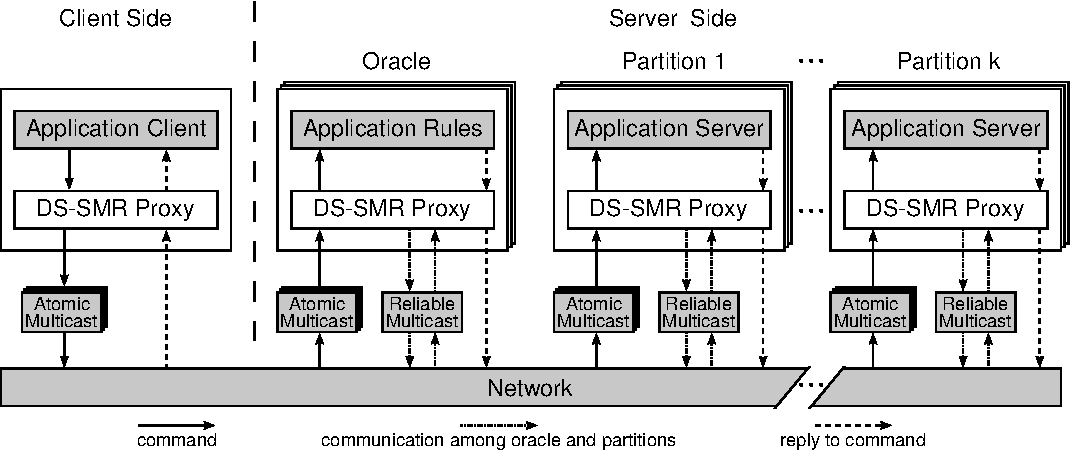
\includegraphics[width=0.8\linewidth]{figures/arch}
%\end{minipage}
%\caption{The architecture of \dssmrlong{}.}
%\label{fig:arch}
%\end{figure*}

